%!TEX TS-program = xelatex
\documentclass[]{friggeri-cv}
\usepackage{afterpage}
\usepackage{hyperref}
\usepackage{color}
\usepackage{xcolor}
\hypersetup{
    pdftitle={},
    pdfauthor={},
    pdfsubject={},
    pdfkeywords={},
    colorlinks=false,       % no lik border color
   allbordercolors=white    % white border color for all
}
\addbibresource{bibliography.bib}
\RequirePackage{xcolor}
\definecolor{pblue}{HTML}{0395DE}

\begin{document}
\header{Yuchen}{Huang}
      {Coder}
      
% Fake text to add separator      
\fcolorbox{white}{gray}{\parbox{\dimexpr\textwidth-2\fboxsep-2\fboxrule}{%
.....
}}

% In the aside, each new line forces a line break
\begin{aside}
    ~
  \section{Tel \& Skype}
    +86 131 2299 0862
    yuchen.huang.purdue
    ~
  \section{Mail}
    \href{mailto:y.huang475@gmail.com}{\textbf{Y.huang475@}{gmail.com}}
    ~
  \section{Tech Interests}
	\textbf{Machine Learning  }
	\textbf{Artificial Intelligence  }
	\textbf{Web Developing  }
	\textbf{Embedded System(IOT)  }  	
	~  	
  \section{Languages}
    \textbf{Python  }
\includegraphics[scale=0.07]{img/3heart.png}
    \textbf{Java  }
\includegraphics[scale=0.07]{img/2heart.png}
    \textbf{HTML/CSS  }
\includegraphics[scale=0.07]{img/2heart.png}
    \textbf{Javascript  }
\includegraphics[scale=0.07]{img/2heart.png}
    \textbf{Bash  }
\includegraphics[scale=0.07]{img/1heart.png}  
    \textbf{Latex  }
\includegraphics[scale=0.07]{img/1heart.png}
    ~
  \section{Toolbox}
  	\textbf{Spring[Boot]}
  	\textbf{Tornado}
  	\textbf{Hystrix}
  	\textbf{ElasticSearch}
  	\textbf{React/Redux}
  	\textbf{Angular}
  	\textbf{AKKA}
  	\textbf{RabbitMQ}
  	\textbf{Zookeeper}
    \textbf{Linux  }
\includegraphics[scale=0.07]{img/2heart.png}
    ~
  \section{Git}
    \href{https://github.com/huang475}{github.com/huang475}
    ~
\end{aside}
~
~
~
\section{Experience}
\begin{entrylist}
  \entry
  	{3/15 - Now}
  	{DevOps Engineer}
  	{Ele.me}
  	{\textbf{CMDB} \textbf{Leader} CMDB is a database for configuration management. It's based on ElasticSearch for easy search and live structure change. Use RabbitMQ for message driven task execution. We also implement Transaction on top of ES, a raw-level lock based on Zookeeper. Also functionality like Trigger and UDF. Though CMDB mainly acts as a rest service, We use React/Redux to construct the Front-end page for easy data lookup. }
  	{\textbf{Operation Centre (EOC)} \textbf{Member} EOC is a job execution framework. The functionality is like SaltStack but supports common language like python, bash for script define. We use zookeeper to support the scalability of core-service. The core-service is written in Python(tornado). }
  	{\textbf{CI/CD System (ELESS)} \textbf{Member} ELESS is a CI/CD system integrating with GitLab/GitHub ,Jenkins, EOC and CMDB. I am responsible for the deployment part. It's basically a gateway service to EOC and CMDB, written in JAVA, mainly in spring[boot]. I use Hystrix for degrading, circuit-breaking and monitoring. And Mysql for some metadata storage. I use persist cache in Redis for degrading is the funny part ... }
  	{\textbf{CMDB Python SDK} \textbf{Alone} It's a small project. I mention it because it's the time I found the awesomeness of Python. It's acting like a ORM, using structure information from CMDB to construct all kinds of Class on the fly.  And it's also the time I notice the importance of API design... }
  	{\textbf{Two Web apps for the Gateway Service I mention above} Both in React/Redux. One is for System admin to do some urgent jobs bypass Eless. The other is the data visualisation of info about all the deployments, charts in Plotly.js. I use some product-ready Material Design / Ant Design components. And I did write a bunch of CSS ... }
  	{\textbf{DBM} \textbf{Alone} It's a mysql management system. Privileges management. Self-define, live edit and manage extra meta info for databases, tables and columns.  Data exploration. Operation tasks scheduling and execution. SQL review workflow. Built with AngularJS, Python(tornado) and ElasticSearch. }
  	{\textbf{DEPLOY}}
  \entry
    {10/14 - 02/15}
    {Software Developer}
    {Epic Systems Corp., Verona, WI, U.S.}
    {\textbf{Web Developing} Working on internal learning web application: Blackboard under C\# .net. \\}
\end{entrylist}
~
~
~
\section{Education}
\begin{entrylist}
  \entry
    {2012 - 2014}
    {Master of Science}
    {Purdue University, West Lafayette, U.S.}
    {\textbf{Electrical and Computer Engineering\\}
Main subjects: Computer architecture, Embedded System, Compilers, Algorithms, Statistic methods, Regression Analysis, ASIC design, Semiconductor.\\}
  \entry
    {2007 - 2011}
    {Bachelor of Engineering}
    {Nanjing University of Posts and Telecommunications, China}
    {\textbf{Electrical and Electronics Engineering\\}
Main subjects: Matematics and Physics, Programming, Operational Research, Telecommunication Systems, Digital and Analogical Electronics.\\}

\end{entrylist}

%\section{Certifications}
%\begin{entrylist}
%  \entry
%    {02/2013}
%    {Intro to Computer Science}
%    {Udacity. E-learning}
%    {\emph{Building a Python Search Engine}}
%\end{entrylist}

\newpage

\begin{aside}
~
~
~
%  \section{Places Lived}
%    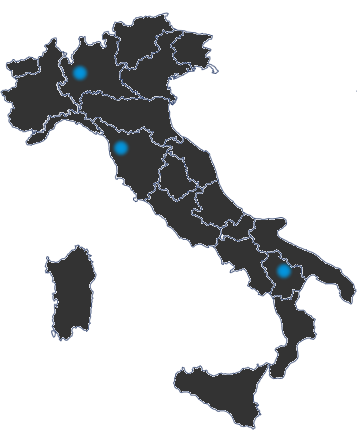
\includegraphics[scale=0.25]{img/italia.png}
%    ~
  \section{Personality}
  	{ISTJ}
    \textbf{Introverted  }
\includegraphics[scale=0.07]{img/3heart.png}
    \textbf{Observant  }
\includegraphics[scale=0.07]{img/1heart.png}
    \textbf{Thinking  }
\includegraphics[scale=0.07]{img/2heart.png}
    \textbf{Judging  }
\includegraphics[scale=0.07]{img/3heart.png}
    \textbf{Assertive  }
\includegraphics[scale=0.07]{img/3heart.png}    
    ~
  \section{Languages}
    \textbf{Chinese  }
\includegraphics[scale=0.07]{img/3heart.png}
    \textbf{English  }
\includegraphics[scale=0.07]{img/2heart.png}
\end{aside}

\section{Projects Details }
\textbf{Blackboard\\}
foo\\
~
\textbf{Sunshine\\}
bar\\
~
\textbf{House Keeper\\}
boo\\
~
\textbf{Lisp Compiler\\}
mii\\
~
\section{Other Info}
For the Italian job market:\\
\emph{Si autorizza il trattamento delle informazioni contenute nel curriculum in conformità alle disposizioni previste dal d.lgs. 196/2003. Si dichiara altresì di essere consapevole che, in caso di dichiarazioni non veritiere, si è passibili di sanzioni penali ai sensi del DPR 445/00 oltre alla revoca dei benefici eventualmente percepiti.}
\\
\begin{flushleft}
\emph{January 14th, 2014}
\end{flushleft}
\begin{flushright}
\emph{Carmine Benedetto}
\end{flushright}

%%% This piece of code has been commented by Karol Kozioł due to biblatex errors. 
% 
%\printbibsection{article}{article in peer-reviewed journal}
%\begin{refsection}
%  \nocite{*}
%  \printbibliography[sorting=chronological, type=inproceedings, title={international peer-reviewed conferences/proceedings}, notkeyword={france}, heading=subbibliography]
%\end{refsection}
%\begin{refsection}
%  \nocite{*}
%  \printbibliography[sorting=chronological, type=inproceedings, title={local peer-reviewed conferences/proceedings}, keyword={france}, heading=subbibliography]
%\end{refsection}
%\printbibsection{misc}{other publications}
%\printbibsection{report}{research reports}

\end{document}
